\appendix

\section{Appendix: The \texttt{VPINN\_HelmholtzImpedanceRF} Network}
\label{app:deeprf}
\autoref{lst:deeprf} includes the code implementation of the proposed network on top of the parent class. In this architecture, we use a local version of ReLU as the activation function of the first hidden layer, and a sinusoidal (hyperbolic tangent) activation function for other hidden layers. The idea is to impose different behaviors for different regions of the domain. \autoref{fig:deeprftrain} shows that without any other consideration, training such a network fails. The solution of the failed training is shown in \autoref{fig:deeprfsol}. Some other similar architectures have been tried out, which also failed. Among those were putting the ReLU activation function only on the last layer, and non-local ReLU activation functions on the first two layers.

\begin{figure}[h!]
    \centering
    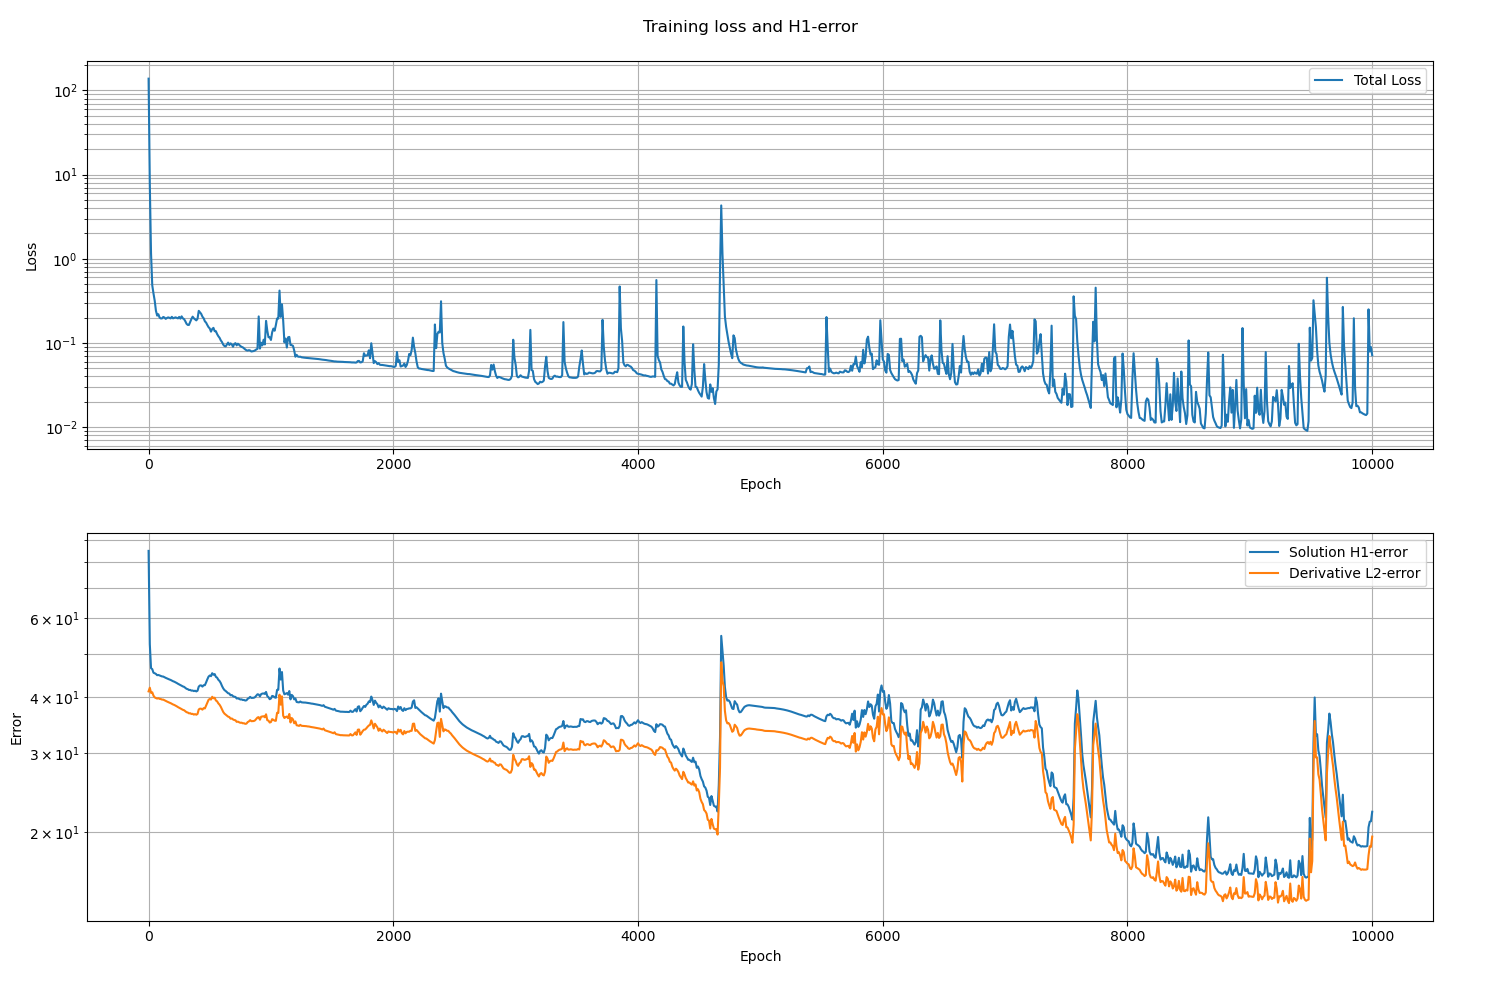
\includegraphics[width = 0.48\textwidth]{img/DeepRF-D004N012K038-training.png}
    \caption{Training loss and solution error of the \texttt{VPINN\_HelmholtzImpedanceRF} network with 4 hidden layers for wave number $k=8.0$.}
    \label{fig:deeprftrain}
\end{figure}

\begin{figure}[h!]
    \centering
    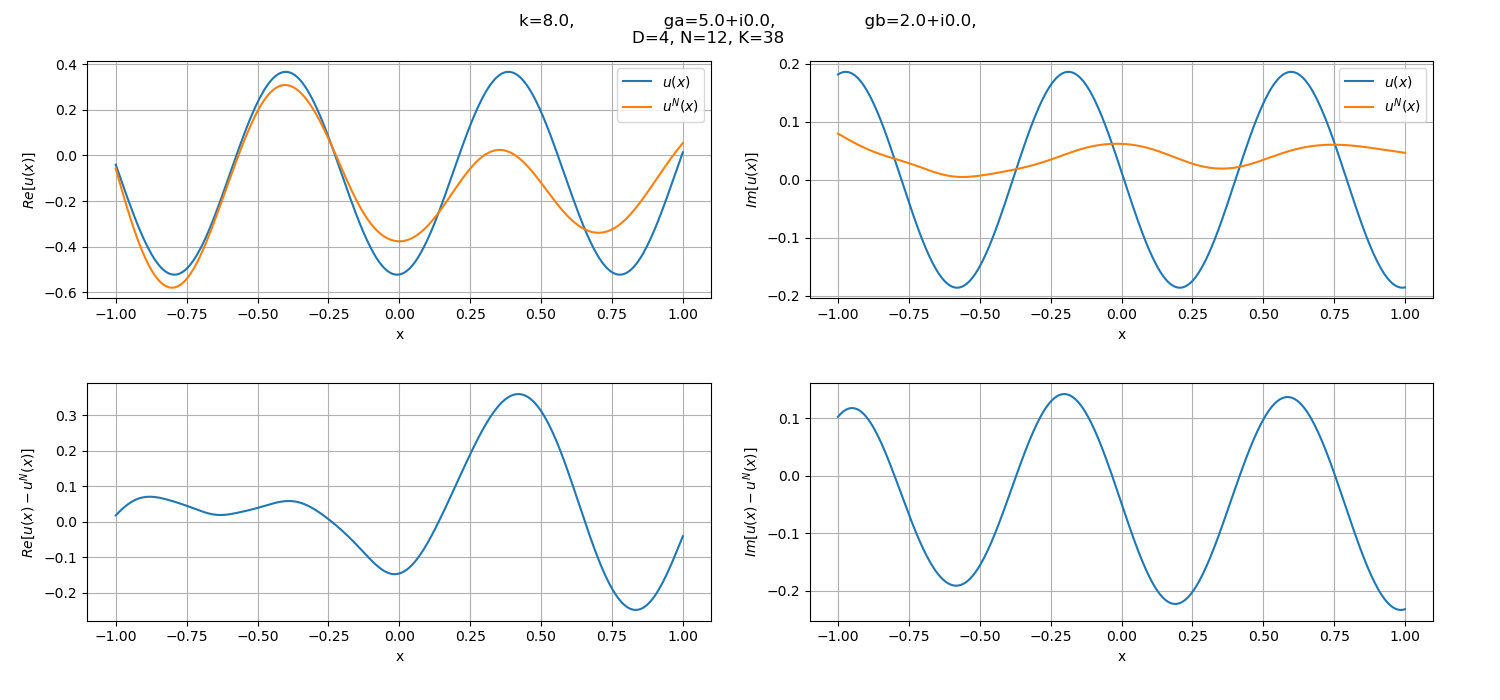
\includegraphics[width = 0.7\textwidth]{img/DeepRF-D004N012K038-sol.png}
    \caption{The solution of the \texttt{VPINN\_HelmholtzImpedanceRF} network with 4 hidden layers for wave number $k=8.0$.}
    \label{fig:deeprfsol}
\end{figure}

\lstinputlisting[
    language=Python,
    style=pythonstyle,
    label={lst:deeprf},
    caption={Code snippet of the \texttt{VPINN\_HelmholtzImpedanceRF} class which inherits from the main \texttt{VPINN\_HelmholtzImpedance} class.}
    ]
{lst/VPINN-HelmholtzImpedanceRF.py}

\section{Appendix: Evolution of the Solution}
\label{app:evolutions}
\autoref{fig:evolutionrandinitsol} illustrates the evolution of the solution of a network architecture that converges to the solution in 30000 epochs. We can see that from the initial random initialization, the network is able to capture the main features of the solution in 2000 epochs, and converges to the final solution in the following 28000 epochs. An interesting observation is that there is a bias from left to right which could also be captured in the initial result of the network (epoch 0). We can see that the solution converges faster in the ranges closer to the left boundary.

The same bias to the left boundary could also be observed in \autoref{fig:evolutionlsinitsol} which illustrates the evolution of solution of the same network with least-squares initialization in the initial 2000 epochs. In \autoref{fig:vpinnslsinitk8}, we can see that the solution error of this network does not improve much with least-square initialization after around epoch 2000. Another observation is that the most of the error comes from the imaginary part of the solution, which is not the case with random initialization.

\begin{figure}[h!]
    \centering
    \begin{subfigure}[b]{0.85\textwidth}
        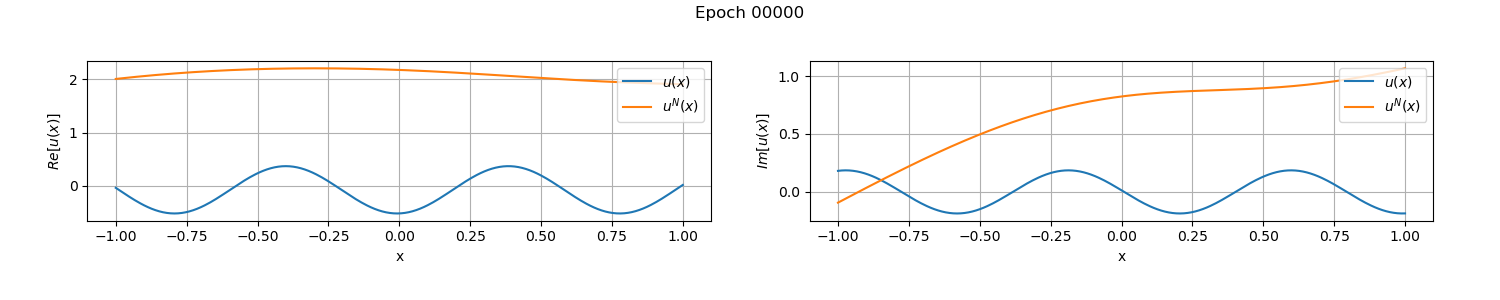
\includegraphics[width=\textwidth]{img/evolution_randinit/sol-00000.png}
    \end{subfigure}
    \vfill
    \begin{subfigure}[b]{0.85\textwidth}
        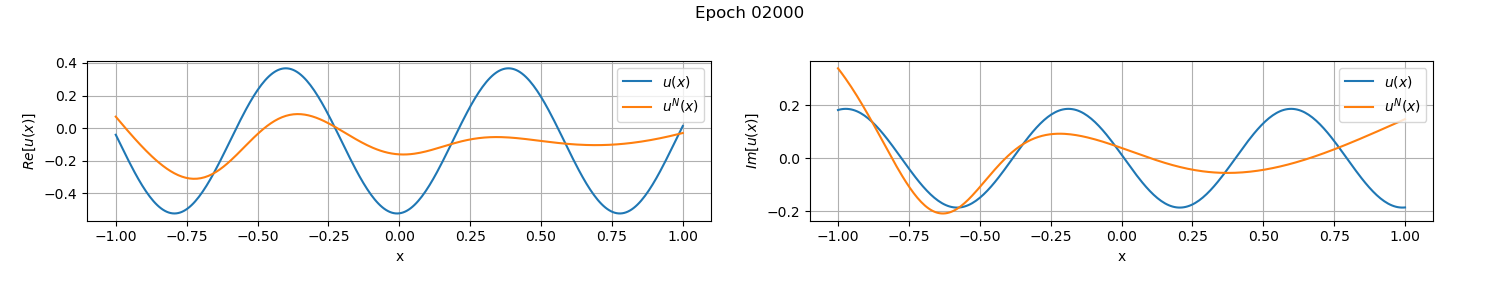
\includegraphics[width=\textwidth]{img/evolution_randinit/sol-02000.png}
    \end{subfigure}
    \vfill
    \begin{subfigure}[b]{0.85\textwidth}
        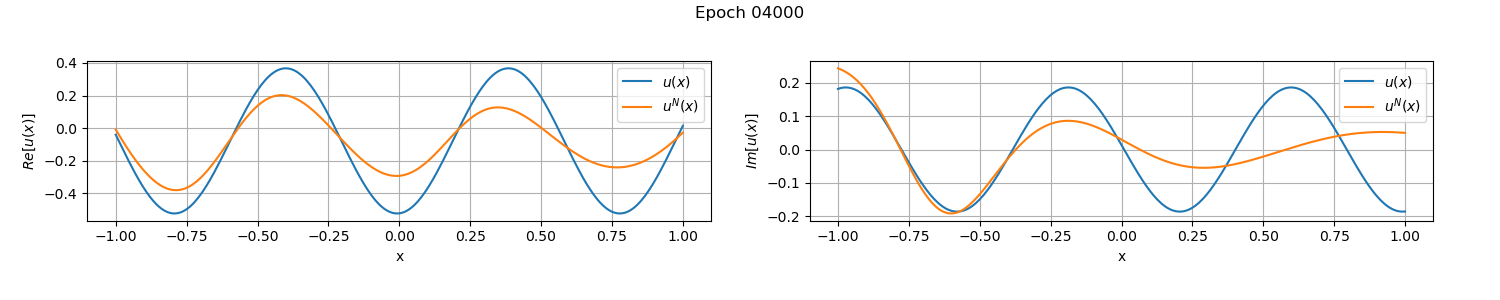
\includegraphics[width=\textwidth]{img/evolution_randinit/sol-04000.png}
    \end{subfigure}
    \vfill
    \begin{subfigure}[b]{0.85\textwidth}
        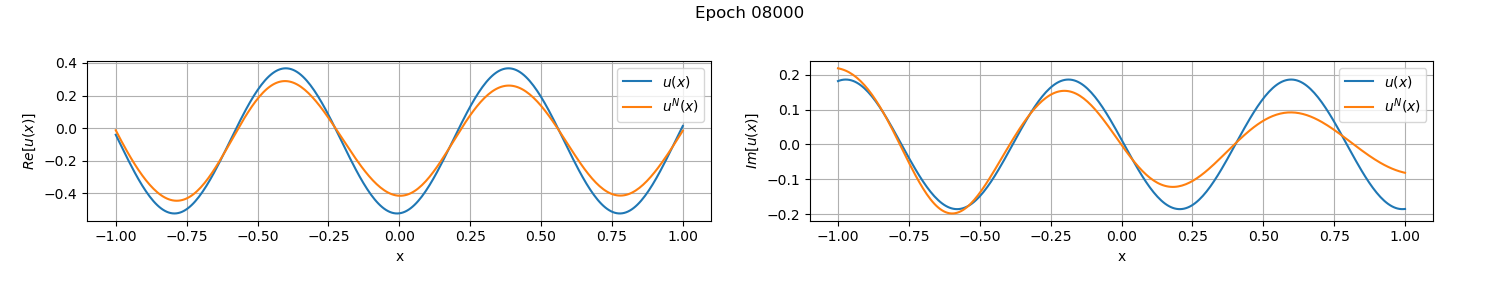
\includegraphics[width=\textwidth]{img/evolution_randinit/sol-08000.png}
    \end{subfigure}
    \vfill
    \begin{subfigure}[b]{0.85\textwidth}
        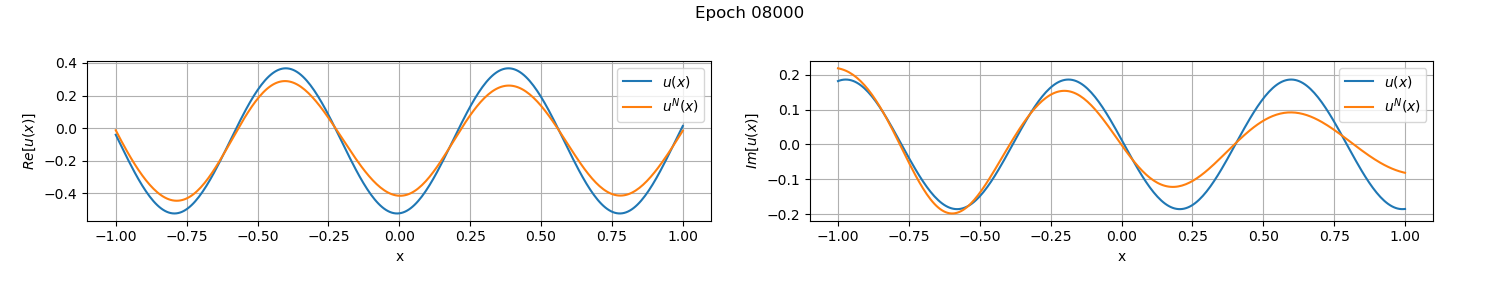
\includegraphics[width=\textwidth]{img/evolution_randinit/sol-08000.png}
    \end{subfigure}
    \vfill
    \begin{subfigure}[b]{0.85\textwidth}
        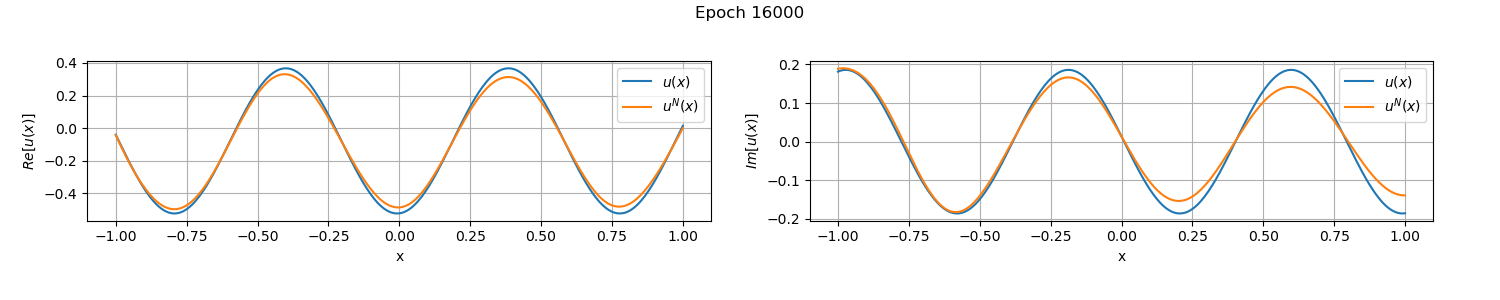
\includegraphics[width=\textwidth]{img/evolution_randinit/sol-16000.png}
    \end{subfigure}
    \vfill
    \begin{subfigure}[b]{0.85\textwidth}
        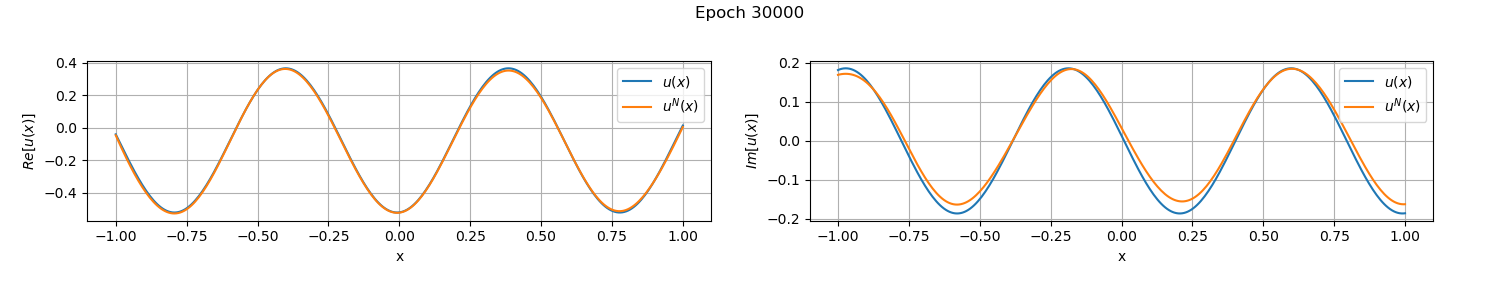
\includegraphics[width=\textwidth]{img/evolution_randinit/sol-30000.png}
    \end{subfigure}
    \caption{The evolution of the solution during the training of a shallow network with 20 nodes and 20 test functions for $k=8.0$.}
    \label{fig:evolutionrandinitsol}
\end{figure}

\begin{figure}[h!]
    \centering
    \begin{subfigure}[b]{0.85\textwidth}
        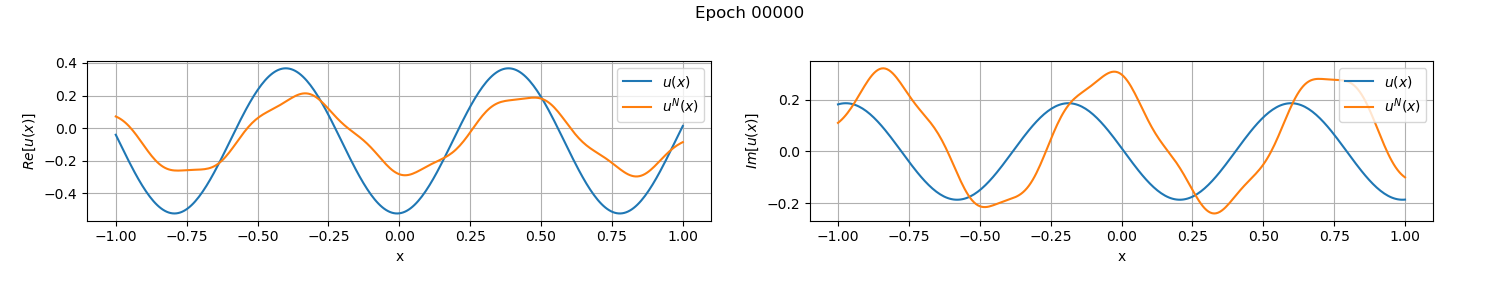
\includegraphics[width=\textwidth]{img/evolution_lsinit/sol-00000.png}
    \end{subfigure}
    \vfill
    \begin{subfigure}[b]{0.85\textwidth}
        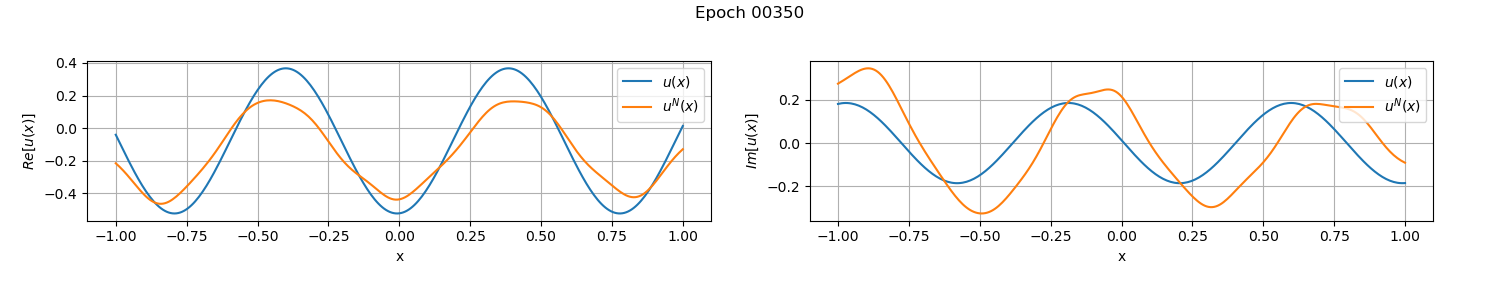
\includegraphics[width=\textwidth]{img/evolution_lsinit/sol-00350.png}
    \end{subfigure}
    \vfill
    \begin{subfigure}[b]{0.85\textwidth}
        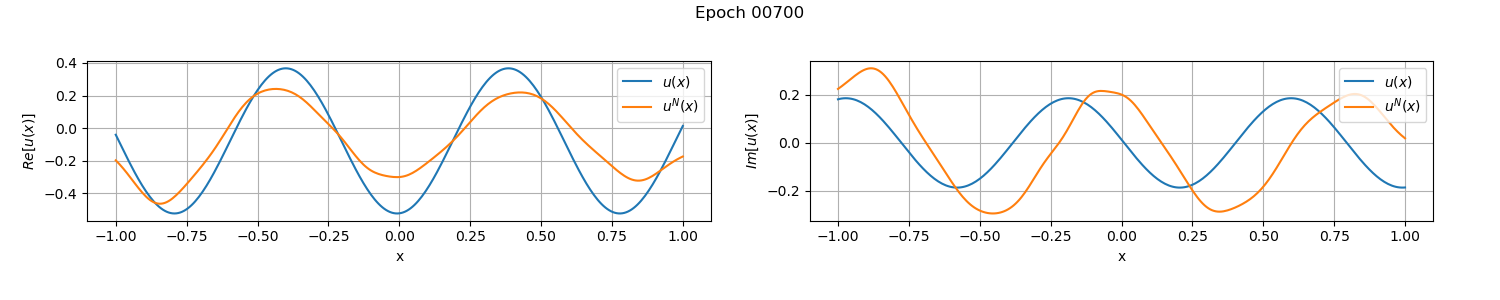
\includegraphics[width=\textwidth]{img/evolution_lsinit/sol-00700.png}
    \end{subfigure}
    \vfill
    \begin{subfigure}[b]{0.85\textwidth}
        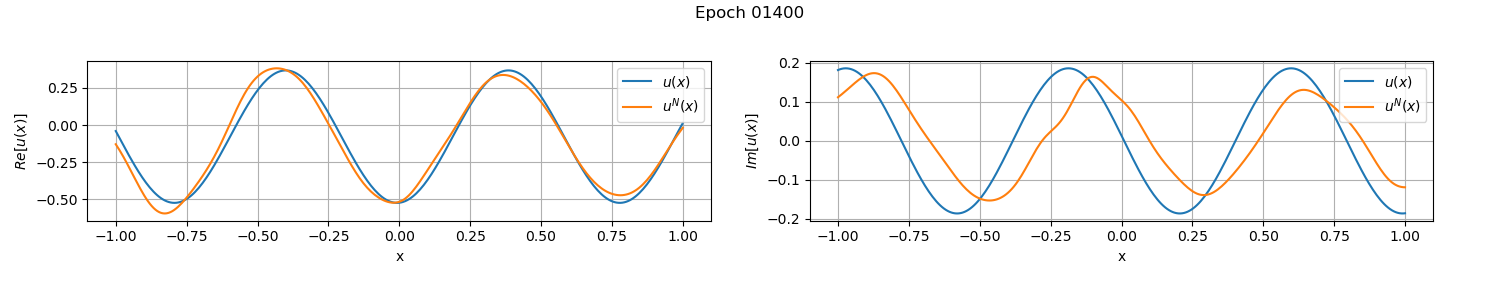
\includegraphics[width=\textwidth]{img/evolution_lsinit/sol-01400.png}
    \end{subfigure}
    \vfill
    \begin{subfigure}[b]{0.85\textwidth}
        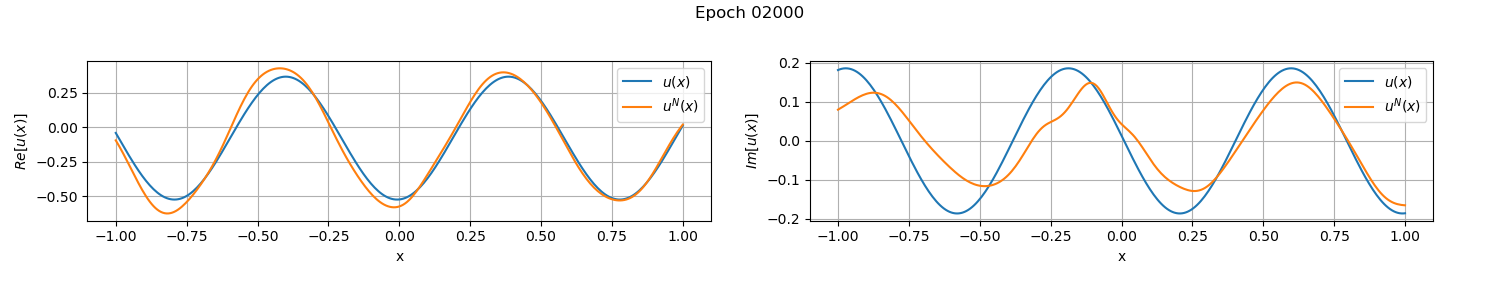
\includegraphics[width=\textwidth]{img/evolution_lsinit/sol-02000.png}
    \end{subfigure}
    \caption{The evolution of the solution during the training of a shallow network with 20 nodes and 20 test functions with least-squares initialization (constant weights) for $k=8.0$.}
    \label{fig:evolutionlsinitsol}
\end{figure}